\documentclass[runningheads]{llncs}

\usepackage{amssymb}
\usepackage{amsmath}
\setcounter{tocdepth}{3}
\usepackage{graphicx}
\usepackage[spanish]{babel}
\usepackage{url}
	

\begin{document}

\mainmatter

\title{Modelo formal para la fusi\'on de Sistemas Multiagentes y Sistemas Gr\'aficos}
\titlerunning{Modelo formal para la fusi\'on de Sistemas Multiagentes y Sistemas Gr\'aficos}

\author{}%Gabriel L\'opez Garc\'ia, Rafael Molina Carmona y Javier Gallego-S\'anchez}
\authorrunning{}%Gabriel L\'opez \and Rafael Molina \and Javier Gallego-S\'anchez}

\institute{}%Grupo de Inform\'atica Industrial e Inteligencia Artificial\\
%Universidad de Alicante, Ap.99, E-03080, Alicante, Spain\\
%\{glopez, rmolina, ajgallego\}@dccia.ua.es}


\maketitle


\begin{abstract}
Se presenta un modelo formal basado en gram\'aticas que unifica lo mejor de los Sistemas Multiagentes y Sistemas Gr\'aficos. Se define los diferentes elementos necesarios para implementar caracter\'isticas esenciales de los Sistemas Multiagentes usando para su visualizaci\'on las herramientas aportadas por los Sistemas Gr\'aficos. Dicho modelo formal nos aporta varias ventajas como la separaci\'on entre la implementaci\'on de la actividad del sistema de la de los dispositivos hardware o la f\'acil reusabilidad de los componentes generados en otros sistemas. Para clarificar el modelo se muestra un caso pr\'actico que implementa la quema forestal de \'arboles por ca\'ida fortuita de rayos.

\end{abstract}

%___________________________________________________________________________

\section{Introducci\'on\label{sec:Introduccion}}

La creciente influencia de los Sistemas Multi-Agentes (SMA) en diversos campos de investigaci\'on originando una importante evoluci\'on en su desarrollo. Por otro lado, el espectacular avance de los Sistemas Gr\'aficos (SG) ha contribuido a que la informaci\'on se presente de forma m\'as amigable, dando a conocer nuevas formas de an\'alisis.

La definici\'on de un agente suele consistir en un conjunto de caracter\'isticas gen\'ericas \cite{Gilbert2008} que hacen dif\'icil su modelado, originando algunos problemas \cite{Axelrod1997},\cite{Gilbert2008}. La representaci\'on visual de los SMA suele tener un car\'acter secundario, aunque existen excepciones \cite{Luke2005,North2005,Wilensky1999}.

En los SMA tiene una vital importancia la relaci\'on de los agentes con su entorno condicionando su comportamiento. Ser\'ia interesante usar el Motor F\'isico (MF) de los SG para esta relaci\'on, sobre todo si est\'a implementado en hardware dedicado. Adem\'as, los SG tratan de modelar la realidad incorporando otros aspectos de comportamiento, en los que un SMA podr\'ia aportar una conducta inteligente.

Hoy en d\'ia existen muchos entornos de trabajo para desarrollar SMA. Se distinguen dos tipos: entornos espec\'ificos que utilizan soluciones basadas en SMA y entornos de trabajo para una arquitectura gen\'erica.

Una de las \'areas donde se est\'a incorporando con mucho \'exito los SMA es en sociolog\'ia (\cite{Axelrod1997,Drogoul,Gilbert2008,Sawyer2005}). Se utilizan soluciones espec\'ificas muy orientadas al estudio sociol\'ogico. Como ejemplos, se puede hacer referencia a entornos que simulan el movimiento de multitudes \cite{Olfati2004,Reynolds2000,Ulicny2001} o el movimiento de estampidas para grupos de individuos \cite{Reynolds2000}. En algunos casos utilizan sistemas gr\'aficos como el descrito en \cite{Reynolds2000} o en \cite{Wilensky1999} con NetLogo.

En el \'ambito de los videojuegos se encuentran usos de SMA aplicados a los juegos\cite{Khoo2002}. Son programados como personajes del juego, que tiene objetivos, estrategias y realizan acciones.

Actualmente est\'a surgiendo una gran variedad de entornos de desarrollo gen\'erico que tienen m\'as o menos la misma filosof\'ia: implementaci\'on de las caracter\'isticas m\'as importantes de los agentes. Se van a destacar dos MASON \cite{Luke2005} y Repast \cite{North2005}, por ser dos entorno que usan SG.

MASON, dise\~{n}ado para un amplio tipo de aplicaciones, define un entorno de simulaci\'on basado en eventos discretos. Los agentes se dividen en dos capas: la capa del modelo que implementa el comportamiento y la capa de visualizaci\'on si se desea su visualizaci\'on.

Repast es un entorno para estudiar simulaciones de grupos. El sistema se basa en modeladores que definen el comportamiento de los agentes. Estos se sit\'uan en el espacio para luego dibujarse en 2D o 3D.

La definici\'on de un modelo que unifique lo mejor de los SMA y los SG supondr\'ia un paso importante dentro de la evoluci\'on de estos tipos de sistemas. Este modelo especificar\'ia todas las caracter\'isticas necesarias para definir un agente, facilitando su visualizaci\'on e interacci\'on.

El presente art\'iculo describe una propuesta que incorpora caracter\'isticas de los SMA y los SG mediante un modelo basado en gram\'aticas.

%___________________________________________________________________________

\section{Objetivos\label{sec:Objetivos}}

Los objetivos pretenden conseguir un modelo que integre los SMA y SG con un lenguaje descriptivo y un sistema de eventos discretos. Para lograr esto se propone:

\begin{enumerate}

\item Dotar al motor gr\'afico de flexibilidad para cambiar la representaci\'on de los elementos sin necesidad de modificar la descripci\'on de la escena. Debe implementar la extracci\'on y uso de la geometr\'ia de los elementos de la escena, necesaria para que los agentes sepan c\'omo es el entorno que les rodea.

\item Definir un MF que se adapte a los diferentes componentes hardware si es que los hay. Podr\'a transmitir informaci\'on del entorno a los agentes, y poder tomar decisiones considerando las limitaciones del entorno.

\item Definir un sistema de interacci\'on para poder manipular los agentes de forma interactiva.

\item Reutilizar los diferentes agentes de forma casi inmediata en cualquier sistema definido.

\end{enumerate}

\section{Dise\~{n}o del sistema\label{sec:DisenodelSistema}}

Un escenario se caracteriza por elementos din\'amicos o agentes que realizan una actividad y elementos est\'aticos. Se visualizan con una secuencia de primitivas y transformaciones definidas en un sistema geom\'etrico representado por un conjunto G.

El concepto de primitiva se debe considerar, no s\'olo como una primitiva de dibujo usual (dibuja una esfera), sino como una acci\'on que se debe ejecutar en un sistema geom\'etrico visual o no. 

Una transformaci\'on es una modificaci\'on del comportamiento de las primitivas. Tienen un \'ambito de aplicaci\'on y s\'olo se aplicar\'a al conjunto de primitivas que se encuentren dentro de ese \'ambito.

El agente es el elemento din\'amico y est\'a compuesto por actividades y un conjunto opcional de estados internos. Toda actividad consiste en un proceso que se ejecuta como reacci\'on a un determinado evento. Puede tener una representaci\'on geom\'etrica que depende de su estado interno definida con transformaciones y primitivas.
	
Un evento ejecuta una actividad y su generaci\'on es independiente del dispositivo que lo genera. Los eventos define las diferentes formas de comunicaci\'on que puede existir en un SMA (agente-agente y agente-entorno).
	
Estos son los principales elementos que componen el sistema. A continuaci\'on, se va a realizar su formalizaci\'on en un modelo matem\'atico que defina de forma precisa sus caracter\'isticas.	

\subsubsection{Formalizaci\'on del sistema\label{sec:FormalizaciondelSistema}}

A cada elemento que compone una escena se le puede asignar un s\'imbolo. Estos contruyen diferentes cadenas que describen una escena mediante una sintaxis definiendo un lenguaje. Una sintaxis se presenta como una gram\'atica \cite{Davis1994} definida por $M~=~<~\Sigma,~N,~P,~S~>$ y determina el lenguaje $L(M)$. Su definici\'on se expresa como:

\begin{enumerate}

\item Sea $\Sigma=P\cup T\cup O\cup A_{s}^{D}$ el conjunto de s\'imbolos terminales donde, P definen las primitivas, T las tranformaciones, O = \{ {\textperiodcentered} ( ) \} el conjunto de separadores y operaciones y $A^{D}_{S}$ es el conjunto que representa agentes que ejecutan actividades cuando reciban los eventos definidos en D, donde D son todos los tipos de eventos generados por el sistema y S el conjunto de los estados internos. As\'i, el agente $a_{s}^{d}$, que est\'a en el estado s, ejecutar\'a la actividad d cuando se produzca un evento $e^{d}$.
	
\item Sea N = \{MUNDO, VARIOSOBJETOS, OBJETO, ACTOR, TRANSFORMACI\'ON, FIGURA\} el conjunto de s\'imbolos no terminales.

\item Sea S = \{MUNDO\} el s\'imbolo inicial de la gram\'atica.

\item Se definen las reglas gramaticales R como:

		\begin{center}
			\begin{tabular}{|l|}
				\hline
					Regla 1.- \textbf{MUNDO} :- VARIOSOBJETOS \\
					Regla 2.- \textbf{VARIOSOBJETOS} :- OBJETO {\textbar} OBJETO {\textperiodcentered} VARIOSOBJETOS\\
					Regla 3.- \textbf{OBJETO} :- FIGURA {\textbar} TRANSFORMACI\'ON {\textbar} ACTOR\\
					Regla 4.- \textbf{ACTOR} :- $a^{d}_{s}$(VARIOSOBJETOS), $a^{d}_{s} \in A^{D}_{S}, d \in D, s \in S$\\
					Regla 5.- \textbf{TRANSFORMACION} :- $t$(VARIOSOBJETOS), $t \in T$\\
					Regla 6.- \textbf{FIGURA} :- $p$, $p \in P$\\
				\hline
			\end{tabular}
		\end{center}

\end{enumerate}

A continuaci\'on se va a asignar a cada regla una funci\'on matem\'atica seg\'un el m\'etodo denotacional para describir sem\'anticas.

\subsubsection{Funci\'on sem\'antica para FIGURA y TRANSFORMACI\'ON (Regla 5 y 6)\label{sec:FuncionPrimitiva}}

	La regla 6 define la sintaxis de una figura como una secuencia de primitivas. Cada primitiva es definida mediante la funci\'on $\alpha$ definida como $\alpha:P\rightarrow G$. Es decir, un s\'imbolo de P ejecutar\'a una primitiva sobre el sistema geom\'etrico G. Esto significa que dependiendo de la funci\'on $\alpha$ y del sistema geom\'etrico G el resultado puede variar. Por ejemplo, G ejecuta primitivas de motor gr\'afico (OpenGL o Direct3D). Otros ejemplos son: c\'alculo de colisiones mediante el c\'alculo de limites, la ejecuci\'on de un sonido, el movimiento de un robot, la transmisi\'on de la escena por una red, etc.	
	
	Los ejemplos anteriores ilustran c\'omo la funci\'on $\alpha$ aporta la abstracci\'on necesaria para homogeneizar las diferentes implementaciones de un SG o proceso geom\'etrico. Con una cadena descriptiva se tienen diferentes formas de extraer informaci\'on que representa cada uno de los elementos que hay en una escena. Esto es importante para relacionar los agentes con el MF. Los procesos de extracci\'on de informaci\'on del entorno se ejecutan en m\'odulos geom\'etricos que componen el MF. La informaci\'on procesada se env\'ia a los agentes para realizar su actividad.
	
	La regla 5 define la sintaxis de una transformaci\'on. Esta transformaci\'on tiene un \'ambito de aplicaci\'on acotado por los s\'imbolos '()'. Se definen dos funciones para describir la sem\'antica de una transformaci\'on, estas son: $\beta:T\rightarrow G$. que se ejecuta al procesar el s\'imbolo '(' y $\delta:T\rightarrow G$ que se ejecuta con el s\'imbolo ')'. Estas dos funciones tienen las mismas caracter\'isticas que la funci\'on $\alpha$ y se definen en el mismo sistema geom\'etrico G.

Con P, T y las funciones $\alpha$, $\beta$, $\delta$, se define una funci\'on que dada una cadena $w$ con s\'imbolos de T y P, ejecute la secuencia de primitivas y transformaciones en el sistema geom\'etrico G. Esta funci\'on es $\varphi$ denominada funci\'on de visualizaci\'on de la escena en un conjunto G y se define como:

\begin{equation}
    \varphi (w) = \left\{
    \begin{array}{ll}
        \alpha(w) & \mathit{Si} \ \ w \in P  \\
        \beta(t); \varphi(v); \delta(t) & \mathit{Si} \ \ w = t(v) \wedge v \in L(M) \\
        \varphi(s); \varphi(t)  & \mathit{Si} \ \ w = s \cdotp t \wedge s, t \in L(M)
    \end{array}\right\}
\end{equation}

La funci\'on no depende de G, s\'olo depende de $\alpha$, $\beta$, $\delta$. Los detalles de implementaci\'on que hay entre un sistema de visualizaci\'on, de c\'alculo geom\'etrico o uno que transporte escenas por una red est\'an encapsuladas en $\alpha$, $\beta$, $\delta$.

\subsubsection{Funci\'on sem\'antica para AGENTE (Regla 4)\label{sec:FuncionAgente}}

La regla 4 referencia a los agentes, la parte din\'amica del sistema. La sem\'antica del agente se describe como una funci\'on denomina funci\'on evolutiva $\lambda$ y se define como: $\lambda: L(M) \times E^D \rightarrow L(M)$ donde $E^D$  es el conjunto de eventos para los dispositivos D (considerando estos dispositivos como cualquier proceso que emite eventos). Al aplicar la funci\'on $\lambda(w,e^{f})$, w se transforma en otra cadena u. La funci\'on $\lambda$ tendr\'a diferente expresi\'on dependiendo de su evoluci\'on. Sin embargo, se puede definir la expresi\'on general como:

\begin{equation}
    \lambda (a^{d}(v),e^{f})=
    \left\{
    \begin{array}{ll}
        u \in L(M) & \mathit{Si}  \ \ f = d \\
        a^{d}_{s}(v)  & \mathit{Si}  \ \ f \neq d
    \end{array}\right\}
\end{equation}

La cadena resultante puede contener al propio agente, puede generar otro evento para la siguiente etapa o cambiar el estado 's' del agente. Los nuevos eventos generados por el agente se acumulan para la siguiente etapa. As\'i, se modela la comunicaci\'on entre agentes tan importante en SMA. En el caso de que el evento no coincida con el evento activador entonces la funci\'on devuelve el mismo agente.

Con la funci\'on $\lambda$ se puede definir un algoritmo recursivo que dado un conjunto de eventos y una cadena, describa la evoluci\'on del sistema. A esta funci\'on se la denomina funci\'on de evoluci\'on del sistema $\eta$. Para su definici\'on se necesita un conjunto de eventos $e^i, e^j, e^k \cdots $ que abreviado se denota como $e^v$, siendo $v \in D^{+}$. Esta funci\'on se define como:

\begin{equation}
    \eta (w, e^v) = \left\{
    \begin{array}{ll}
        w   & \mathit{Si}  \ \ w \in P  \\
        t(\eta (v, e^v))    & \mathit{Si}  \ \  w = t(v)  \\
        \underset{\forall f \in v}{ \prod }(\lambda (a^{d}_{s} (\eta (y, e^v)), e^f))    & \mathit{Si}  \ \ w = a^{d}_{s}(y)\\
        \eta (s, e^v) \cdot \eta (t, e^v)   & \mathit{Si}  \ \  w = s \cdot t
    \end{array}\right\}
\end{equation}

El operador $\underset{\forall f \in v}{ \prod }(\lambda (a^{d}_{s} (\eta (y, e^v)), e^f))$ realiza la concatenaci\'on de las cadenas generadas por $\lambda$. Para cadenas que s\'olo son transformaciones y primitivas, el sistema se queda como est\'a, formando s\'olo parte del entorno.

Para la visualizaci\'on de un agente se necesita primero transformar los agentes a cadenas de primitivas y transformaciones. Este proceso se realiza con un tipo especial de funciones $\lambda$. A estas funciones se las denominaran funciones de visualizaci\'on y su definici\'on es: $\theta: L(M) \times E^V \rightarrow L(E)$ donde $E^V$ son los eventos que se generan en la visualizaci\'on, y L(E) es el lenguaje L(M) sin agentes. La expresi\'on de la funci\'on de visualizaci\'on se define como:

\begin{equation}
    \theta (a^d(v), e^f) =
    \left\{
    \begin{array}{ll}
        u \in L(E) & \mathit{Si}  \ \ f = d \wedge d \in V \\
        \epsilon  & \mathit{Si}  \ \ f \neq d
    \end{array}\right\}
\end{equation}

Se puede observar que existen peque\~{n}as diferencias entre $\lambda$ y $\theta$. La primera es que $\theta$ devuelve cadenas que pertenecen a L(E). La segunda es que si no coincide con el evento se devuelve una cadena vac\'ia no teniendo representaci\'on para eso evento.
	
El tipo de evento V es importante y no se corresponde con ning\'un dispositivo de entrada en concreto, si no que es un evento que se encarga de establecer los diferentes tipos de vista que tiene el sistema o procesos geom\'etricos.

Al igual que con $\lambda$, se define un algoritmo para $\theta$ que devuelve una cadena $z \in L(E)$, dada una cadena $w \in L(M)$ y un conjunto de eventos $e^v$ con $v \in V^+$, y $V \subseteq D $. A esta funci\'on se le denomina funci\'on de visualizaci\'on $\pi$ ($\pi: L(M) \times E^V \rightarrow L(E)$) y se define como:

\begin{equation}
   \begin{array}{c}
    \pi (w, e^v) = \left\{
    \begin{array}{ll}
        w   & \mathit{Si}  \ \ w \in P^+  \\
        t(\pi (y, e^v))     & \mathit{if}  \ \  w = t(y)  \\
        \underset{\forall f \in v}{ \prod }(\theta (a^v (\pi(y, e^v)), e^f))    & \mathit{Si}  \ \ w = a^v(y) \\
        \pi (s, e^v) \cdot \pi (t, e^v)    & \mathit{Si}  \ \  w = s \cdot t
    \end{array}\right\} \\
   \end{array}
\end{equation}

\subsubsection{Funci\'on sem\'antica para OBJETO, VARIOSOBJETOS y MUNDO (Regla 1,2,3)\label{sec:FuncionAgente}}

Las funciones sem\'anticas de estas reglas descomponen las cadenas en subcadenas y dependiendo de si es un agente, una transformaci\'on o una primitiva ejecutan las funciones antes especificadas. Se debe observar que las primitivas que no son generadas por los agentes con la funci\'on de visualizaci\'on representan la parte est\'atica del sistema, o lo que es lo mismo, el entorno donde se desarrolla la actividad del sistema.

%___________________________________________________________________________

\subsection{Actividad y eventos\label{sec:ActividadYEventos}}

En los SMA se deben establecer mecanismos para que la actividad dentro del sistema pueda ser modelada. Esta actividad se realiza en los agentes y se activan con eventos. 

{\itshape
Se define $e^{d}_{c}$ como el evento de tipo $d \in D$ que se va a ejecutar bajo la condici\'on $c$ y tiene como datos $e$.

Se define $e^{d}$ como el evento de tipo $d \in D$ y tiene como datos $e$.
}

Se puede observar que el origen de la creaci\'on de los eventos no es importante y s\'i el tipo de evento y sus datos. Esto no quiere decir que en el evento no se pueda incluir datos que identifiquen qui\'en env\'ia el mensaje. Por ejemplo, en la comunicaci\'on entre dos agentes  los eventos pueden contener informaci\'on sobre qui\'en envi\'o el mensaje. De esta manera se establece un sistema gen\'erico de comunicaci\'on que puede implementar KMQL, FIPA \cite{Genesereth1995} o cualquier otro.
	
\subsubsection{Dispositivos de entrada y generadores de eventos\label{sec:DipositivosDeEntradaYGeneradoresDeEventos}}

	Se desea establecer una independencia entre el sistema y los dispositivos que generan eventos (hardware o software). Para ello, se especifica una funci\'on que genera los eventos que se necesitan para hacer reaccionar al sistema. Esta funci\'on define un mecanismo para dar informaci\'on del entorno a los agentes. Este elemento es el generador de eventos y su definici\'on es:
	
	{\itshape
		Se define como $C^d(t)$ al generador que crea los eventos del tipo d en el instante t, siendo $d \in D$ donde D es el conjunto de todos tipos de eventos que pueden ser generados por el sistema.
	}

	Se debe destacar que los eventos se generan en un instante t por motivos de sincronizaci\'on. El generador es la parte dependiente del dispositivo de entrada encapsulada en una \'unica funci\'on, asilando esta dependencia del sistema.
	
	Para que no se produzcan ambig\"uedades se va a establecer un orden de prioridad entre los generadores, de tal manera que, dados dos generadores $C_i$ y $C_j$ con $i < j$, si crean dos eventos del mismo tipo entonces prevalecer\'a el evento creado por $C_i$ sobre el $C_j$. 
	
	El proceso para la obtenci\'on de los eventos producidos por todos los dispositivos de entrada y sus generadores asociados se define como:
	
	{\itshape
		Si $C^*$ es el conjunto de todos los generadores de eventos del sistema y la funci\'on $E(C^*,t)$ recolecta todos los eventos de todos los generadores entonces:
		
\begin{eqnarray*}
E(C^{*},t)=\left\{ \begin{array}{ll}
e(z,C_{i}(t)) & \mathit{Si}\ z=E(C^{*}-C_{i},t)\\
\epsilon & \mathit{Si}\ C^{*}=\emptyset\end{array}\right\}  
& 
con
& 
e(z,e^{i})=\left\{ \begin{array}{ll}
z\cdot e^{i} & \mathit{Si}\ e^{i}\notin z\\
z & \mathit{Si}\ e^{i}\in z\end{array}\right\} 
\end{eqnarray*}
}

Tanto con los generadores de eventos como con los eventos que genera los agentes, se puede modelar todo lo relacionado con los procesos de comunicaci\'on que existen en los SMA (tanto entre dos agentes como entre agente y entorno).

\subsection{Algoritmo del sistema\label{sec:Algoritmo del sistema}}

Una vez definidos todos los elementos implicados en el modelo que gestionar\'a un SMA, se puede establecer el algoritmo que ejecuta todo el sistema:

\begin{center}
\begin{tabular}{lll}
\begin{tabular}{|ll|}
    \hline
    1. & $w = w_o$ ; $t = 0$ \\
    2. & $e^* = E(G^*, t)$ \\
    3. & $e^v =$ eventos de $e^*$ donde $v \in V^+$ \\
    4. & $e^u = e^* - e^v$ \\
    5. & $w_{next} = \eta(w, e^u)$ \\
    6. & $v =  \pi(w, e^v)$ \\
    7. & $g = \varphi(v)$ \\
    8. & $w = w_{next}; \ \ t = t + 1$ \\
    9. & Si $w = \epsilon$ entonces Ir a 12 \\
    10. & Ir a 3 \\
    11. & Fin \\
\hline
\end{tabular}
	 & & 
\begin{small}
\begin{tabular}{p{0.5\linewidth}}
	$w_o$ Cadena inicial del sistema.\\
	
    $e^*$ Eventos generados en el frame $t$.\\    
    
	$C^*$ = \{Todos los generadores de eventos\}\\
	
	$D$ = \{Todos los eventos del sistema\}\\
	
    $V$ = \{Todos los eventos visuales\} $V \subseteq D$\\
    
    $e^v$ Eventos visuales generados.\\

    $e^u$ Eventos no visuales generados.\\

    $g$ dispositivo de salida gr\'afica.\\
\end{tabular}
\end{small}
\end{tabular}
\end{center}

	En primer lugar se inicializa el sistema ($w_o$ y $t = 0$).	 Los pasos 2, 3 y 4 gestionan los eventos del sistema. En el paso 5 se llama a la funci\'on de evoluci\'on para calcular el siguiente frame. En los pasos 6 y 7 se visualiza el frame. En 8 se prepara para la siguiente iteraci\'on y el paso 9 se mira si se ha llegado al final (cadena vac\'ia, resultado de un evento especial) si no es as\'i se pasa a 3.
	
	Se puede destacar que al no compartir datos los pasos 6 y 7-8 pueden ser facilmente paralelizable optimizando el algoritmo de forma significativa.
	
%___________________________________________________________________________
\section{Caso Pr\'actico
\label{sec:casoPractico}}
%___________________________________________________________________________

Este ejemplo es una aplicaci\'on que simula incendios forestales causados por la ca\'ida aleatoria de rayos. Se busca la mejor distribuci\'on de \'arboles para reducir el n\'umero de \'arboles quemados \cite{John2007}. El sistema basicamente consiste en un agente que define el bosque. Este agente crea otros agentes que definen \'arboles y relampagos. Dada una posici\'on $(i,j)$ de un tablero 2D, representado por el bosque, se puede situar un \'arbol con una probabilidad $g$ o un rayo con una probabilidad $f$. En el caso de que caiga un rayo sobre un \'arbol este arder\'a y todos los que esten a su alrededor provocando una reacci\'on en cadena. El ejemplo tiene que definir 4 elementos principales: eventos, generadores de eventos, agentes y primitivas gr\'aficas.

Los eventos son los causantes de la actividad del sistema. Los evento definidos para este ejemplo son:

\begin{itemize}
    \item $t$: Se genera cada cierto tiempo t.

    \item $c$: Crea un \'arbol en la posici\'on $(i, j)$.

    \item $f$: Crea un rayo en la posici\'on $(i, j)$.

    \item $e$: Elimina el \'arbol en la posici\'on dada $(i, j)$.

    \item $b$: Quema un \'arbol en la posici\'on $(i, j)$.

    \item $v$: Dibuja la escena usando una librer\'ia gr\'afica (en este caso OpenGL).
\end{itemize}

El siguiente paso se debe definir los generadores de eventos.

\begin{itemize}
	\item \textit{Generador de eventos de tiempo} ($C_{time}$): Es responsable de las animaciones del sistema. Cada cierto tiempo $t$, se genera un evento $e^t$.

	\item \textit{Generador de elementos del bosque} ($C_{forest}$): Genera eventos para crear \'arboles ($e^{c}$) con provabilidad $g$ y rel\'ampagos ($e^{f}$) con probabilidad $f$.

	\item \textit{Generador de visualizaci\'on} ($C_{visualization}$): Captura las \'ordenes de dibujado y produce un evento para dibujar la escena en el sistema gr\'afico.
\end{itemize}

El cuadro \ref{table2} muestra las primitivas y las transformaciones para dibujar la escena. Las funciones 
${\alpha}$, ${\beta}$ y ${\delta}$ definen el comportamiento de ambas. En este caso implementan el dibujado en la librer\'ia gr\'afica OpenGL.
\begin{table}[h]
\begin{center}
\begin{small}
\begin{tabular}{lll}

\begin{tabular}{|l|l|}
	\hline \itshape Primitivas & \itshape Descripci\'on\\
	\hline $TR$   & Dibuja un \'arbol\\
	\hline $TR_b$ & Dibuja un \'arbol quem\'andose\\
	\hline $FA$   & Dibuja un rayo\\
	\hline $BO$   & Dibuja un tablero de NxN \\
	\hline
\end{tabular}
 & & 
\begin{tabular}{|l|l|}
	\hline \itshape Transformaciones & \itshape Descripci\'on\\
	\hline $D_{i,j}$ & Desplazar (i,j)\\
	\hline $S_{s}$ & Escalar (s)\\
	\hline
\end{tabular}

\end{tabular}
\end{small}
\caption{\label{table2} (Izquierda) Primitivas, (Derecha) Transformaciones}
\end{center}
%%\end{table}

%%\begin{table}[h]
\begin{center}
\begin{small}
\begin{tabular}{|p{0.08\linewidth}|p{0.15\linewidth}|p{0.73\linewidth}|}

	\hline 
	\itshape Agente & 
	\itshape Descripci\'on & 
	\itshape Funci\'on ${\lambda}$ y ${\pi}$\\
	\hline

	\ \ $BO$ & 
	\ Bosque &
	\begin{tabular}{lll}
		$\lambda(BO^{cfe}, e^{i})$ & $=$ & $\left\{
		\begin{array}{ll}
			TR_{s1}^{t=1} \cdot BO^{cfv} 	& \ \ \ i = c \\
			FA^{t=1}   \cdot BO^{cfv} 	& \ \ \ i = f \\
			BO^{cfe} 			& \ \ \ i = e \\
			BO^{cfe} 			& \ \ \ i \neq c,f,e
		\end{array}
		\right\}$ \\
		
		$\pi (BO^{v}, e^{i})$ & $=$ & $\left\{
	    \begin{array}{ll}
    		BO        	& \ \ \   i = v \\
    		\epsilon 	& \ \ \   i \neq v
		\end{array}
		\right\}$
	\end{tabular}   \\
	
	\hline

	\ \ $TR$ & 
	\ \'Arbol &
	\begin{tabular}{lll}
		$\lambda(TR_{st}^x, e^{i})$ & $=$ & $\left\{
		\begin{array}{ll}
			TR_{s1}^{t+1} 		& i = t \wedge t+1 \leqslant N \wedge s = s1 \\		
			TR_{s2}^{b} 		& i = t \wedge t+1 > N \wedge s = s1 \\
			TR_{s3}^{t=1} \wedge \Delta Nbo^{b} 		& i = b > N \wedge s = s2 \\
			TR_{s3}^{t+1} 		& i = t \wedge s = s3 \\
			\Delta e^{e} 		& i = t \wedge	t+1 > N  \wedge s = s3 \\
			TR_{st}^{t} 		& i \neq t \wedge	i \neq b \\
		\end{array}
		\right\}$ \\
	
    	$\pi (TR_{st}^{v}, e^{i})$ & $=$ & $\left\{
	    \begin{array}{ll}
    		D_{(i, j)}( S_{s} (TR) )	& \ \ \   i = v \wedge st = s1 \\
    		D_{(i, j)}( TR )		& \ \ \   i = v \wedge st = s2 \\
	    	D_{(i, j)}( S_{s^{-1}} (TR) )	& \ \ \   i = v \wedge st = s3 \\
    		\epsilon 			& \ \ \   i \neq v
		\end{array}\right\}$
	\end{tabular}   \\

	
	\hline

	\ \ $FA$ & 
	\ Rayo &
	\begin{tabular}{lll}
		$\lambda (FA^{t}, e^{i})$ & $=$ & $\left\{
		\begin{array}{ll}
			FA^{t+1} 		& \ \ \  i = t \wedge t+1 \leqslant N \\
			\Delta e^{b} 		& \ \ \  i = t \wedge t+1 > N \\
			FA^{t} 			& \ \ \  i \neq t 
		\end{array}
		\right\}$ \\

	    $\pi (FA^{v}, e^{i})$ & $=$ & $\left\{
	   	\begin{array}{ll}
	    	D_{(i, j)}(FA)			& \ \ \   i = v \\
    		\epsilon 			& \ \ \   i \neq v
		\end{array}
		\right\}$
	\end{tabular}   \\
	
	\hline
\end{tabular}
\end{small}
\caption{\label{table4} Definici\'on de agentes}
\end{center}
\end{table}

El cuadro \ref{table4} define los agentes mediante su funci\'on de evoluci\'on $\lambda$ y su representaci\'on gr\'afica por su funci\'on $\pi$.

El agente que define un \'arbol ($TR$) tiene tres estados internos $st = \{s1, s2, s3\}$ donde $s1$ corresponde al estado de creciendo, $s2$ a crecido y $s3$ a en llamas. Esto es un ejemplo de como un agente puede terner diferente representaci\'on seg\'un su estado interno. La llamada de la funci\'on $Nbo$ env\'ia eventos de quemado $e^b$ a todos sus vecinos provocando la reacci\'on en cadena (comunicaci\'on agente-agente). Un ejemplo de comunicaci\'on entorno-agente es entre el bosque y el generador $C_{forest}$ que cambia el entorno.

$S$ representa el factor de escala en el crecimiento de un \'arbol y depende del estado actual del agente. El valor es definido por la expresi\'on $s = t / N$, donde $N$ es el total del n\'umero de frames. En el caso de $TR_b$ el factor de escala es decrementado $s^{-1}$. En general, todas las animaciones depende de $t$ que modifica el estado actual del agente y su representaci\'on.

Por \'ultimo, la cadena inicial se define como: $w_{0}=B^{cfe}$.

\begin{figure}[htb]
  	\centering
	\begin{tabular}{cc}
  		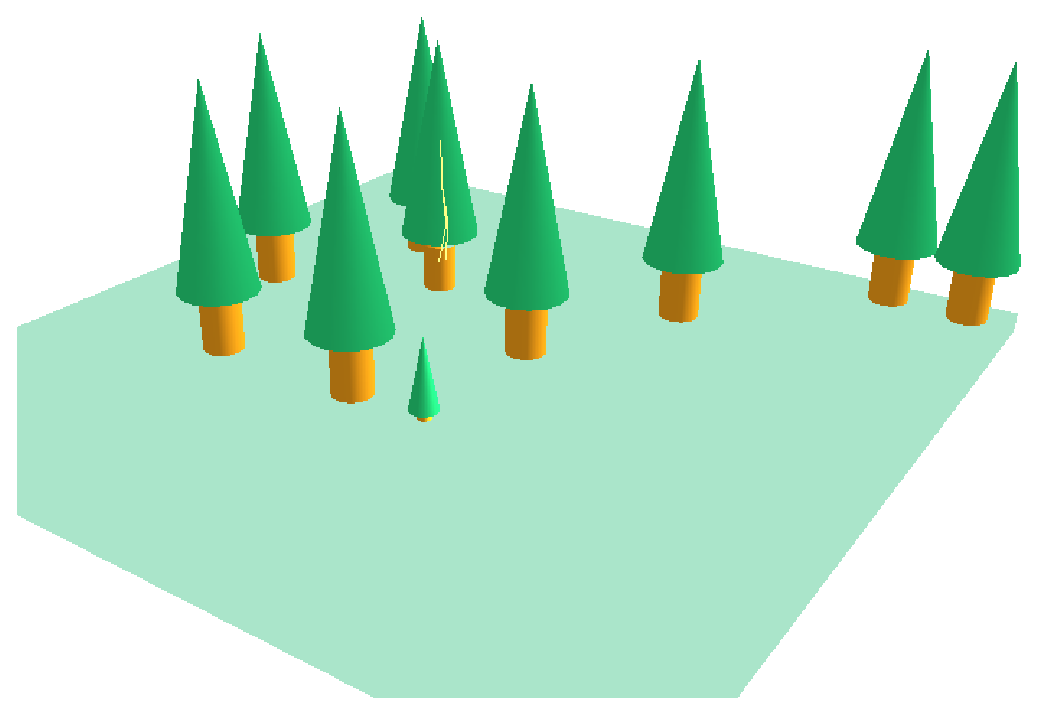
\includegraphics[width=5cm]{img/figure1.eps}
	\end{tabular}
 	\caption{\label{fig:ejemplo} Vista del bosque}
\end{figure}


%___________________________________________________________________________

\section{Conclusiones y trabajos futuros \label{Conclusiones}}

Se ha dise\~nado un sistema de comunicaci\'on entre los procesos geom\'etricos que definen un MF y los agentes que componen una escena mediante el generador de eventos.

El uso de un lenguaje para la descripci\'on de los elementos de la escena y la independencia del sistema gr\'afico hace que estas cadenas descriptivas puedan ser reutilizadas.

	Este modelo abre diferentes expectativas que podr\'an ser exploradas en el futuro. Por ejemplo, se podr\'ian estudiar el desarrollo de algoritmos de modificaci\'on gen\'etica. Dado un agente como $r^{abc}$, se podr\'ia definir una funci\'on de evoluci\'on que dado un evento pueda producir la reproducci\'on de $r$ pero con modificaciones en la cadena de eventos. Es decir, se podr\'ia reproducir como la cadena $r^{ab}$ o incluso incluir otros eventos como $r^{abd}$.
	
	Una posible \'area de aplicaci\'on del modelo podr\'ia ser en rob\'otica. Un robot puede comportarse como un agente o un conjunto de ellos. Los diferentes sensores pueden definir generadores de eventos que tratar\'ian la se\~{n}al y pasar a los agentes la informaci\'on procesada.
	
En definitiva, se ha pretendido dar una soluci\'on que integra lo mejor de los SMA y SG y cuya aplicaci\'on puede aplicarse en toda la gran variedad de problemas.

\begin{thebibliography}{0}

\bibitem{Axelrod1997} 
\textsc{Robert Axelrod}
\newblock Advancing the Art of Simulation in the Social Sciences
\newblock \emph{Simulating Social Phenomena}, Springer, 1997

\bibitem{Drogoul} 
\textsc{Alexis Drogoul, Jacques Ferber, Christophe Cambier}
\newblock Multi-agent Simulation as a Tool for Analysing Emergent 
\newblock \emph{Processes in Societies} 1992

\bibitem{Genesereth1995} 
\textsc{Michael R. Genesereth, Steven P. Ketchpel}
\newblock Software Agents
\newblock \emph{Communications of the ACM} 1995

\bibitem{Gilbert2008} 
\textsc{Nigel Gilbert}
\newblock Agent-Based Models
\newblock \emph{SAGE Publications} 2008

\bibitem{Gratch2002} 
\textsc{Jonathan Gratch, Jeff Rickel, Elisabeth André, Justine Cassell, Eric Petajan, Norman I. Badler}
\newblock Creating Interactive Virtual Humans:Some Assembly Required.
\newblock \emph{IEEE Intelligent Systems} July-August 2002

\bibitem{John2007} 
\textsc{John H.Miller}
\newblock Complex Adaptative Systems 
\newblock \emph{Princeton University Press} 2007

\bibitem{Khoo2002} 
\textsc{Aaron Khoo, Robert Zubek}
\newblock Applying Inexpensive AI Techniques to Computer Games
\newblock \emph{IEEE Intelligent Systems} July-August 2002

\bibitem{Luke2005} 
\textsc{Sean Luke, Claudio Cioffi-Revilla, Liviu Panait, and Keith Sullivan}
\newblock MASON: A New Multi-Agent Simulation Toolkit
\newblock \emph{Simulation Vol. 81, SAGE Journals} 2005

\bibitem{Maes1995} 
\textsc{Pattie Maes, Trevor Darrell, Bruce Blumberg, Alex Pentland}
\newblock The ALIVE System:Wireless, Full-body Interaction with Autonomous Agents, 
\newblock \emph{ACM Multimedia Systems, Vol.5, No.2, pp.105-112} 1997

\bibitem{North2005} 
\textsc{M.J. North, T.R. Howe, N.T. Collier, J.R. Vos}
\newblock The Repast Simphony Runtime System 
\newblock \emph{Conference on Generative Social Processes, Models, and Mechanisms, Proceedings of the Agent} 2005

\bibitem{Olfati2004} 
\textsc{Reza Olfati-Saber}
\newblock Flocking for Multi-Agent Dynamic Systems:Algorithms and Theory 
\newblock \emph{IEEE Transactions on Automatic Control} 2004

\bibitem{Reynolds2000} 
\textsc{Craig Reynolds}
\newblock Interaction with Groups of Autonomous Characters 
\newblock \emph{Game Developers Conference} 2000

\bibitem{Rhyne2000} 
\textsc{Theresa-Marie Rhyne}
\newblock Computer Games’Influence on Scientific and Information Visualization
\newblock \emph{Entertainment Computing} 2000

\bibitem{Sawyer2005} 
\textsc{R. Keith Sawyer}
\newblock Social Emergence: Societies As Complex Systems 
\newblock \emph{Cambridge University Press} 2005

\bibitem{Ulicny2001}
\textsc{Branislav Ulicny, Daniel Thalmann}
\newblock Crowd simulation for interactive virtual environments and VR training systems 
\newblock \emph{Computer Animation and Simulation, Springer} 2001

\bibitem{Wilensky1999} 
\textsc{Wilensky, U., NetLogo}
\newblock User Manual, 1999

\bibitem{Wachsmuth1995} 
\textsc{Ipke Wachsmuth, Yong Cao}
\newblock Interactive Graphics Design with Situated Agents 
\newblock \emph{Graphics and Robotics} 1995

\bibitem{Davis1994}
\textsc{Davis Martin D.,Sigal R.,Weyuker E. J.}:
\newblock \emph{Computability, Complexity, and Languages, Fundamentals of Theoretical Computer Science}, 2nd~ed.
\newblock San Diego: Elsevier Science, 1994.

\end{thebibliography}

\end{document}
